\documentclass[letterpaper, 12pt]{article}
\usepackage[round]{natbib}
\bibliographystyle{apalike}
\usepackage[margin=1in]{geometry}
\usepackage{enumitem}
\usepackage{csquotes}
\usepackage{graphicx}
\usepackage{float}
\usepackage{svg}


\usepackage{xcolor} % 
\newcommand{\bca}[1]{\textcolor{blue}{BA: #1}} % Blair
\newcommand{\jl}[1]{\textcolor{purple}{JL: #1}} % Li
\newcommand{\todo}[1]{\textcolor{red}{#1}} % Things to fix.

\begin{document}
%\title{Proposal for the application to UTSC Postdoctoral Fellowship %Program}
%\author{Jiangtian Li}
%\maketitle

A central challenge in developing a theory of how the mind processes language is how the meanings of ambiguous words are resolved. Approximately 85\% of the words in the world's languages are ambiguous, yet humans resolve most ambiguities correctly and effortlessly \citep{KleinRepresentationPolysemousWords2001}.  For example, in the phrase ``A prime minister wields significant power'' a reader has no difficulty evoking a ``political power'' interpretation as opposed to an ``electrical power'' interpretation.  However, how ambiguity is resolved remains open, despite having received attention from interdisciplinary researchers (including philosophers such as myself, as well as linguists, and psychologists), and despite the game-changing role that a theory of ambiguity resolution could have for artificial intelligence.

My proposal builds upon the latest insights from several disciplines to develop and test a novel account of ambiguity resolution. My philosophy background makes me appreciate the fundamental weakness of a cognitive system without grounded and referential information connected to the outer world \citep{searleMindsBrainsPrograms1980}. Meanwhile, from the psycholinguistics and neuroscience literatures (including work by my proposed advisor, Professor Blair Armstrong), I will draw on recent findings demonstrating that building in additional neurobiological plausibility into simulations are essential for simulating ambiguity resolution \citep{Armstrong2016Disparatesemanticambiguity}.

RESEARCH PLAN: My research plan starts from a (relatively) simple neural network model and gradually increasing the complexity of this model to achieve better performance. It quantifies how each new level of complexity improves over simpler models. Such complexity is not achievable until the recent development in training methods and hardwares. These models will be trained on databases of images and their associated captions, such as the Common Objects in Context dataset, so that they will learn to see objects while simultaneously processing their verbal description. And each model will be tested against published data in the psycholinguistics literature which will serve as the ``gold standard'' for successfully modeling human ambiguity resolution abilities \citep{Eddington2015Howmeaningsimilarity}.

1.  Language-only model. The first model will be trained only on the verbal caption in the COCO dataset, and provides a baseline for how much disambiguating information can be extracted from text alone \citep{beekhuizenWhatCompanySemantically2018}.

2.  Integrated vision-and-language model.  The second model will add a visual processing system to the model developed in (1), and will serve as a first validation for how visual information can provide additional constraint on word meaning than the prior model.

3.  More biologically plausible integrated model.  The third model will focus on how several key principles from cognitive and systems neuroscience could further enhance performance in the model: 3(a) Addition of an attention mechanism. Humans do not process all of the information their eyes take in equally well, rather, they focus attention on one part of the visual field. 3(b) More realistic cortical connectivity. In human neural networks, neurons send excitatory OR inhibitory information, NOT both as in the artificial neural networks; and there are fewer connections between different brain regions compared to artificial networks. Prior work \citep{laszloPSPsERPsApplying2014, Armstrong2016Disparatesemanticambiguity} has established that these principles critically shape what type of information shapes network performance, including word disambiguation. 

EXPECTED OUTCOME AND IMPLICATIONS: I will revolutionize how ambiguity is thought about in many fields by merging insights from several fields to develop an account that would not emerge from any one discipline in isolation. The understanding of how ambiguity is resolved will have a huge impact on studying how language interacts with contexts, both the narrower linguistic and broader social-cultural.  Finally, the project can be potentially patented, if successful, to allow its free use to academics as well as its incorporation into industry, like Microsoft, Facebook, Google, etc, including building better “bots” to communicate with customers online, and better automated screening of user content for remarks that are inappropriate or discriminatory.

\begin{figure}[h]
\begin{center}
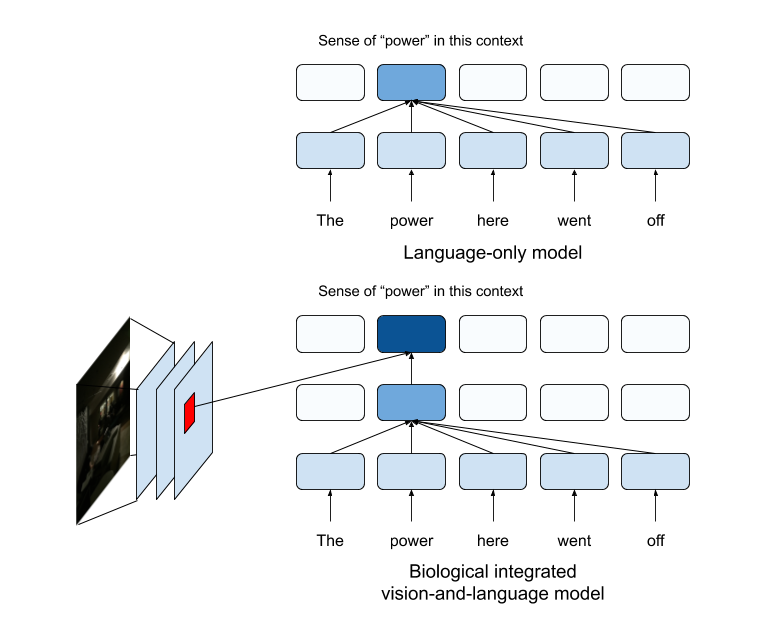
\includegraphics[width=0.7\textwidth,keepaspectratio]{model_figure}
\end{center}
    \caption{Computational models that are going to be build in this project.}
\end{figure}

\newpage
% \bibliography{/Users/jiangtianli/MyWriting/Mybib.bib}
\bibliography{Proposal_for_fellowship.bib}
\end{document}
